% Capítulo 3
    \chapter{JGOOSE}
        \label{cap:jgoose}
        % intro
            Neste capítulo,
            é apresentada a ferramenta JGOOSE (\emph{Java Goal into Object Oriented Standard Extension}).
            %
            % Visão geral
            Inicialmente, na seção \ref{cap:jgoose-sec:overview},
                    % histórico
                    % diretrizes e passos
                são apresentados os principais conceitos, objetivos e as diretrizes que norteiam os processos de mapeamento de modelos organizacionais i* para casos de uso UML da ferramenta.
                Ainda nessa seção, também é apresentado um resumo histórico das versões ao longo dos anos e as principais contribuições de outros autores.
            % Projeto e Arquitetura
            Em seguida, na seção \ref{cap:jgoose-design},
                é analisada a organização estrutural da ferramenta, mostrando os impactos da proposta deste trabalho (\ferramenta{}) na estrutura e processos da JGOOSE.
        % [end]

    \section{Visão Geral}
        \label{cap:jgoose-sec:overview}
        % intro
            A JGOOSE é uma ferramenta de auxílio no mapeamento de modelos organizacionais para modelos funcionais \cite{vicente2006}.
            Essa ferramenta implementa seus processos guidados pelas diretrizes propostas por Santander \cite{santander2002integrando} e é com base nessas diretrizes que a ferramenta interpreta os modelos organizacionais do framework i* e gera os casos de uso UML, apresentando-os no \emph{template} proposto por Cockburn \cite{cockburn2001writing}.
            Com essa ferramenta, é possível derivar casos de uso com base nas intencionalidades associdadas aos atores de um ambiente organizacional.

            Na subseção a seguir, apresentaremos as diretrizes e passos da proposta de Santander \cite{santander2002integrando}, para posteriormente melhor compreender o funcionamento da ferramenta JGOOSE.
            E, na subseção seguinte (\ref{cap:jgoose-subsec:historico}), será apresentado um resumo histórico sobre as principais mudanças já ocorridas no projeto JGOOSE.

        \subsection{Diretrizes e Passos}
            O conjunto de diretrizes e passos propostos por Santander \cite{santander2002integrando} são a essência dos processos realizados pela ferramenta JGOOSE.
            É com base nessas diretrizes e passos que a ferramenta realiza o mapeamento de modelos organizacionais i* para modelos funcionais de Caso de Uso UML.
            A seguir, são descritas brevemente essas diretrizes e passos \cite{brischke2012melhorando}:

            \begin{enumerate}
                \item[1º Passo:] Descoberta de atores;
                \begin{enumerate}
                    \item[Diretriz 1:] todo ator em i* deve ser analisado sob um possível mapeamento para ator em caso de uso.
                    \item[Diretriz 2:] deve-se analisar se o ator em i* é externo ao sistema computacional pretendido, pois atores em caso de uso nunca são partes do sistema. Caso o ator seja externo ao sistema, o mesmo é considerado candidato a ator em Casos de Uso.
                    \item[Diretriz 3:] se o ator i* candidato tiver pelo menos uma dependência com o sistema computacional pretendido, esse deve ser um ator em caso de uso.
                    \item[Diretriz 4:] atores em i* relacionados através do mecanismo ISA, ou seja, com heranças de suas atividades nos modelos organizacionais e mapeados individualmente para atores em casos de uso (aplicando diretrizes 1, 2 e 3), serão relacionados no diagrama  de casos de uso através do relacionamento do tipo <<\emph{generalization}>>.
                \end{enumerate}

                \item[2º Passo:] Descoberta de Casos de Uso;
                \begin{enumerate}
                    \item[Diretriz 5:] para cada ator descoberto para o sistema no 1º passo, devemos observar todas as suas dependências (\emph{dependum}) como \emph{dependee} em relação ao ator que representa o sistema computacional pretendido (\emph{depender}), visando descobrir casos de uso para o ator.
                    \item[Subdiretriz 5.1:] deve-se analisar as dependências do tipo objetivo associadas com o ator e mapeadas diretamente para casos de uso.
                    \item[Subdiretriz 5.2:] deve-se avaliar as dependências do tipo tarefa associadas com o ator. Se um ator depende de outro ator para realizar uma tarefa, deve-se investigar se esta tarefa necessita ser refinada em subtarefas. Este tipo de tarefa pode ser mapeada para caso de uso.
                    \item[Subdiretriz 5.3:] deve-se avaliar as dependências do tipo recurso associadas com o ator. Se um ator depende de outro ator para obter um recurso, por que o mesmo é requerido? Se para esta resposta existe um objetivo, o mesmo será candidato a ser um objetivo de um caso de uso para este ator.
                    \item[Subdiretriz 5.4:] deve-se avaliar as dependências do tipo objetivo-soft associadas com o ator. Normalmente uma dependência do tipo objetivo-soft em i* é um requisito não-funcional associado ao sistema pretendido.
                    \item[Diretriz 6:] analisar a situação especial na qual um ator de sistema (descoberto seguindo as diretrizes do passo 1) possui dependências (como \emph{depender}) em relação ao ator em i* que representa o sistema computacional pretendido ou parte dele (ator $\rightarrow$ \emph{dependum} $\rightarrow$ sistema computacional).
                    \item[Diretriz 7:]  classificar cada caso de uso de acordo com seu tipo de objetivo associado: contextual, de usuário ou de subfunção.
                \end{enumerate}

                % \item[3º Passo:] Descoberta e descrição do fluxo principal e alternativo dos Casos de Uso.
                \item[3º Passo:] Especificação de Caso de Uso;
                \begin{enumerate}
                    \item[Diretriz 8:] analisar cada ator e seus relacionamentos no modelo de Razões Estratégicas (SR) para extrair informações que possam conduzir à descrição de fluxos principais e alternativos, bem como, pré-condições e pós-condições dos casos de uso descobertos para o ator.
                    %
                    Para isso precisamos analisar os subcomponentes em uma ligação de decomposição de tarefa mapeando-os para passos na descrição do cenário primário (fluxo principal) de casos de uso.
                    %
                    Também devemos analisar ligações do tipo meio-fim mapeando os meios para passos alternativos na descrição de casos de uso.
                    %
                    \item[Diretriz 9:] investigar a possibilidade de derivar novos objetivos de casos de uso a partir da observação dos passos nos cenários (fluxos de eventos) dos casos de uso descobertos.
                    %
                    \item[Diretriz 10:] Desenvolver o diagrama de casos de uso utilizando os casos de uso descobertos e os relacionamentos do tipo <<\emph{include}>>, <<\emph{extend}>> e <<\emph{generalization}>> usados para estruturar as especificações dos casos de uso.
                \end{enumerate}
            \end{enumerate}
        %

        \subsection{Resumo Histórico}
            \label{cap:jgoose-subsec:historico}
            % intro
                Desde a sua primeira versão \cite{vicente2006}, a ferramenta JGOOSE passou por várias melhorias e aprimoramentos.
                Mudanças essas que variam desde a refatoração de código fonte (Classes e \emph{Packages} Java) até alterações na interface gráfica do usuário \cite{brischke2011melhorando}.
                A seguir, é apresentado um resumo sobre a origem da JGOOSE e as principais alterações já realizadas na ferramenta.
            % 
            \begin{itemize}
                \item \textbf{GOOSE} -
                    % Marcelo Brischke
                    A \emph{Goal into Object Oriented Standard Extension} (GOOSE), foi a ferramenta que antecedeu à JGOOSE.
                        Implementada com a linguagem de programação \emph{Object Pascal} e com a extensão \emph{Rational Rose} por Marcelo Brischke \cite{brischke2005desenvolvimento}, possuía dependências das ferramentas OME e Rational Rose.
                    Devido a dependência dessa última, que é uma solução proprietária, a GOOSE foi distribuída sob uma licença educacional.
                    Analisando sob aspectos técnicos e funcionais, a ferramenta não contemplava todas as diretrizes propostas por Santander \cite{santander2002integrando}. Mais especificamente, as diretrizes 5.7, 7 e 9 não eram satisfeitas pelo processo do sistema \cite{brischke2005desenvolvimento}.

                \item \textbf{JGOOSE versão 2006} -
                    % André Abe Vicente
                    Desenvolvida por André Abe Vicente \cite{vicente2006},
                        a nova implementação passou a ser na linguagem Java e, com isso, foi atribuído o nome de JGOOSE (\emph{Java Goal into Object Oriented Standard Extension}).
                    Por ser em uma nova linguagem de programação, todo o projeto teve que ser re-implementado em Java.
                    Entre outros aspectos, a solução continuou dependente da ferramenta OME, contudo não utilizava mais a extensão Rational Rose.
                    Além disso, essa versão contou com a implementação da subdiretriz 5.4, aperfeiçoamento de outras subdiretrizes e novas funcionalidades de auxílio ao usuário no processo de mapeamento \cite{vicente2006}.

                \item \textbf{JGOOSE versão 2011} -
                    % Mauro Brischke
                    Melhorada por Mauro Brischke \cite{brischke2011melhorando},
                        a nova versão contempla a implementação de três diretrizes faltantes: 8, 9 e 10.
                    Também foi fruto desse trabalho a implementação da exportação dos casos de uso no formato XMI, melhorando a comunicação com outras ferramentas como a StarUML.
                    Nessa versão, foi implementado soluções que permitiram o usuário da ferramenta a realizar um refinamento manual dos casos de uso gerados, bem como visualizar graficamente os casos de uso na forma de imagens estáticas.

                \item \textbf{JGOOSE versão 2013} - 
                    Essa versão está em fase de desenvolvimento por Diego Peliser \cite{peliser2013aprimorando} e visa a correção de alguns \emph{bugs} na aplicação das diretrizes e a otimizações de código (algoritmos), bem como melhorias na interface gráfica e na documentação.
            \end{itemize}

        % finalizacao comparativa? - Com base nesse resumo histórico...
    % [end]

    \section{Projeto e Arquitetura}
        \label{cap:jgoose-design}
            Conforme o resumo histórico, a JGOOSE sofreu várias alterações ao longo dos anos.
            Entretanto, nenhuma dessas alterações influenciaram de forma significativa o fluxo de dados tradicional da ferramenta, mantendo como base as diretrizes e passos propostos por Santander \cite{santander2002integrando}.
            A figura \ref{fig:jgoose-arquitetura} foi apresentada por Brischke \cite{brischke2011melhorando} como sendo a represetanção da arquitetura da ferramenta JGOOSE.

            \begin{figure}[h!]
                \centering
                    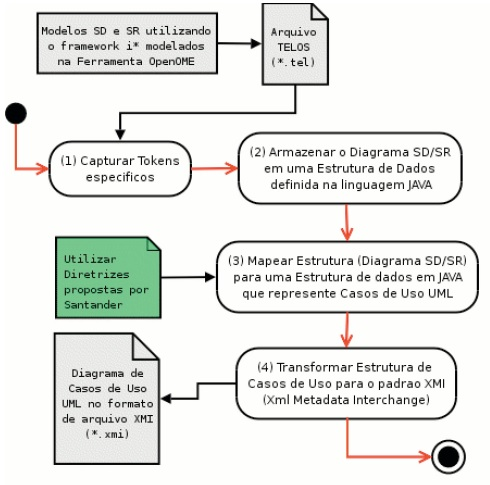
\includegraphics[scale=1]{Figuras/jgoose-arquitetura.jpg}
                    \caption{Figura apresentada por Brischke como ``Arquitetura da ferramenta JGOOSE Demonstrando o seu Funcionamento'' \cite{brischke2011melhorando}.}
                    \label{fig:jgoose-arquitetura}
            \end{figure}

            A figura \ref{fig:jgoose-arquitetura} foi analisada e refeita sobre os conceitos de DFD (\emph{Data Flow Diagram}) nos modelos de Gane e Sarson \cite{gane1977structured}.
            Antes de apresentar o novo diagrama sobre o fluxo de dados da JGOOSE, precisamos entender os elementos do DFD usados nesse diagrama.
            
            Nesse tipo de modelo (DFD), temos os seguintes elementos (apresentados na figura \ref{fig:dfd-captions}):

            % def. elementos DFD
                \begin{figure}[h!]
                    \centering
                        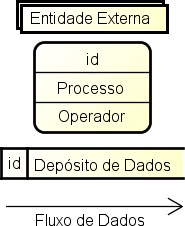
\includegraphics[scale=0.8]{Figuras/dfd-captions.png}
                        \caption{Elementos da notação Gane e Sarson \cite{gane1977structured} de DFD.}
                        \label{fig:dfd-captions}
                \end{figure}

                \begin{itemize}
                    \item \textbf{Entidade Externa}
                        - representam elementos de fora do sistema, mas que comunicam-se com ele.
                        São fontes de entradas de dados para o sistema ou destinos para as saída dos dados e contém apenas o \emph{nome} da entidade na sua representação.
                    %
                    \item \textbf{Processo} 
                        - representa uma transformação dos dados de entrada em dados de saída.
                        Contém um \emph{id}entificador único, um \emph{nome} do processo e o \emph{operador} do processo.
                    %
                    \item \textbf{Depósito de Dados}
                        - representa um repositório de dados no sistema, podendo ser tanto em banco de dados quanto em arquivos.
                        Contém um \emph{id}entificador único e o \emph{nome} do depósito de dados.
                    %
                    \item \textbf{Fluxo de Dados}
                        - representam canais através do qual passam as informações. Aplica-se uma etiqueta para representar os dados que ``passam'' por esse canal.
                \end{itemize}

            % diagrama de contexto
                Em modelos de DFD, existem os chamados \emph{diagramas de contexto DFD}, que expressam, em mais alto nível de abstração, a interação entre \emph{entidades externas} e somente um \emph{processo} do sistema \cite{gane1977structured}. Esse único processo deve resumir e representar as funções principais do sistema.
                Com base nesses conceitos,
                    foi construído um diagrama de contexto DFD (figura \ref{fig:dfd-context}) para representar o fluxo de dados entre a \emph{entidade externa} OME3, o \emph{processo} realizado pelo \emph{operador} JGOOSE e a \emph{entidade externa} StarUML.
                
                    \begin{figure}[h!]
                        \centering
                            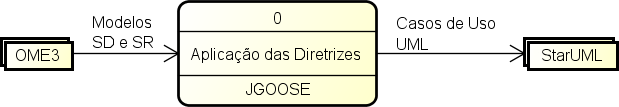
\includegraphics[scale=0.8]{Figuras/dfd-context-3.png}
                            \caption{Diagrama de contexto da Ferramenta JGOOSE.}
                            \label{fig:dfd-context}
                    \end{figure}

            % diagrama DFD
            Para melhor representar o fluxo de dados da JGOOSE, um diagrama com maiores detalhes nos processos foi construído e apresentados na figura \ref{fig:dfd-detail-1}.
            Esse diagrama visa representar a ``antiga estrutura'' da figura \ref{fig:jgoose-arquitetura} na forma de DFD tradicional, mostrando a \emph{entidade externa} OME3, os \emph{processos} da atual JGOOSE e \emph{entidade externa} StarUML.

            \begin{figure}[h!]
                \centering
                    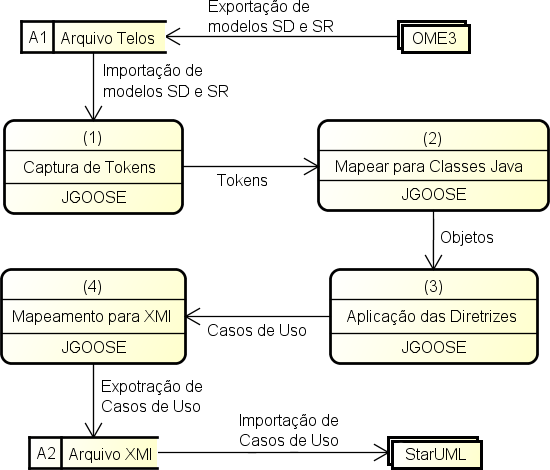
\includegraphics[scale=0.8]{Figuras/dfd-detail-1.png}
                    \caption{Diagrama de Fluxo de Dados da Ferramenta JGOOSE.}
                    \label{fig:dfd-detail-1}
            \end{figure}

        \subsection{Impacto da \ferramenta{}}
            Para realizar a integração da \ferramenta{} com a JGOOSE, serão necessárias algumas modificações do fluxo de dados original da JGOOSE.
            Conforme a proposta deste trabalho, que trata da manipulação de diagramas SD e SR,
                os processos ``(1) - Captura de Tokens - JGOOSE'' e ``(2) - Mapear para Classes Java - JGOOSE''
                deverão ser gerenciados pela \ferramenta{}.
                Dessa forma, um novo diagrama de fluxo de dados com a \ferramenta{}, é apresentado a seguir (figura \ref{fig:dfd-proposta}):
                \begin{figure}[h!]
                    \centering
                        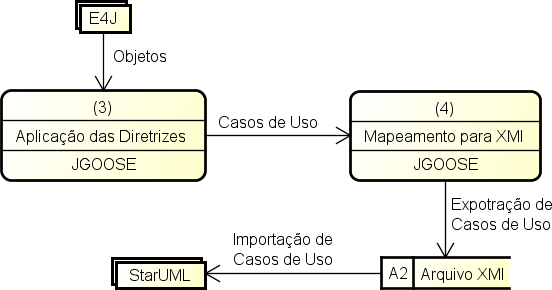
\includegraphics[scale=0.8]{Figuras/dfd-proposta.png}
                        \caption{Novo DFD da ferramenta JGOOSE, após integração com \ferramenta{}.}
                        \label{fig:dfd-proposta}
                \end{figure}

            Após a integração entre as duas ferramentas, não será mais possível executar diretamente a JGOOSE, pois essa passa a ser um módulo interno da \ferramenta{} (mais detalhes dessa integração serão apresentados na seção \ref{cap:proposta-sec:maven} do capítulo \ref{cap:proposta}).
            O processo de mapeamento se iniciará dentro da \ferramenta{} e, após as rotinas de mapeamento da estrutura em iStarML para a estrutura legada da JGOOSE, a linha de execução do programa passa a ser de responsabilidade da JGOOSE.
            Somente após o fechamento da interface da JGOOSE é que a linha de execução retorna ao gerenciamento da \ferramenta{}.

            Com isso, um novo diagrama de contexto DFD, onde a \ferramenta{} passa a ser o processo principal, é apresentada na figura \ref{fig:dfd-context-e4j}.
                \begin{figure}[h!]
                    \centering
                        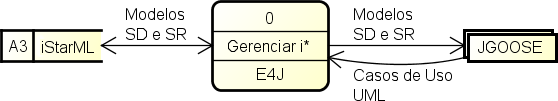
\includegraphics[scale=0.8]{Figuras/dfd-context-e4j.png}
                        \caption{Novo diagrama de contexto com a \ferramenta{} sendo o processo principal.}
                        \label{fig:dfd-context-e4j}
                \end{figure}
    % [end]

    \section{Considerações Finais do Capítulo}
        Considerando os processos que serão de responsabilidade da \ferramenta{},
            é conveniente pensar na incorporação da JGOOSE à \ferramenta{}, pois é com a \ferramenta{} que se inciam os processos que antecedem o mapeamento da JGOOSE.
        Dessa forma, a JGOOSE passará a cuidar especificamente das rotinas (diretrizes e passos) de mapeamento da estrutura (objetos e classes) i* para a estrutura de casos de uso UML, enquanto a \ferramenta{} trata dos processos iniciais de manipulação dos diagramas organizacionais.
        Em trabalhos futuros, pode-se estudar a viabilidade da alteração de algumas estruturas e rotinas da JGOOSE para usar as mesmas estruturas (objetos e classes) que a \ferramenta{}.
        Vale ressaltar que a integração \textbf{não afetará} a forma com a qual a JGOOSE realiza suas funções de mapeamento. Apenas deixará de executar suas rotinas de interpretação dos modelos organizacionais feitos em TELOS.
    % [end]

% bibliography, just for auto-link in sublime text
% before compile main.tex, comment line below
% \bibliography{../referencias/unioeste,../referencias/commons,../referencias/books,../referencias/tecnologias,../referencias/istar}
